\documentclass[english]{article}
\usepackage[T1]{fontenc}
\usepackage[latin9]{inputenc}
\usepackage{color}
\usepackage{babel}
\usepackage{amsmath}
\usepackage{graphicx}
\usepackage{ragged2e}
\justifying
\begin{document}

\title{\Large{\textbf{Air Cargo Optimization}}}
\author{DDS - RWTH Business School}
\date{April 30th, 2018}

\maketitle

\begin{flushleft}
\textbf{\underline{\large{Introduction}}}:

Unit Load Devices (ULDs) are unloaded from an aircraft by the ground handling agent and placed in a drop zone (not part of planning puzzle). Each ULD has a scheduled arrival and at a later stage an actual arrival time. From the drop zone the ULDs need to be transported to a breakdown zone (BD zone), which are located at different places of the airport, have different capacity and handling times within the zone. Next to this some kind of goods are only allowed in some BD zones. A ULD can be loaded with different types of goods (cooled goods, animals,..), so depending on this a BD zone needs to be chosen.

$\newline$

\noindent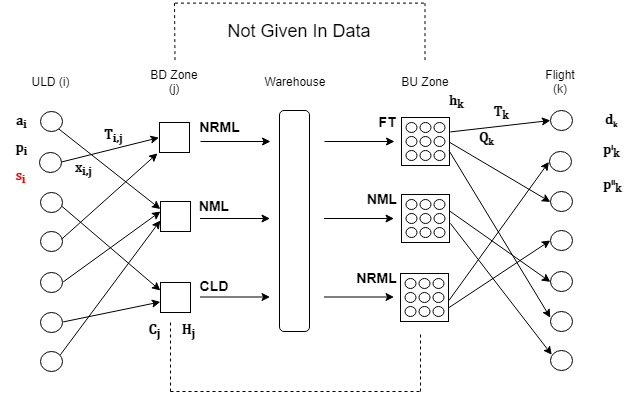
\includegraphics[width=13cm]{Aircargo_overall.png}\qquad

\pagebreak

\textbf{\underline{\large{Arrival}}}:

Let each ULD ${\color{black}i\in{\color{black}I = \{1,2,3,\dots,n\}}}$

${\color{black}a_{i}}$ - Arrival time of each ULD ${\color{black}i}$

$\textcolor{black}{s_{i}}$ - Idle time spent by ULD i at drop zone

$\textcolor{black}{p_{i}}$ - Priority of ULD i

$\newline$

\textbf{\underline{\large{Break Down (BD) Zones}}}: $\textcolor{black}{j\in J = \{1,2,3,\dots,m\}}$

$\newline$

\textbf {From the drop zone the ULDs need to be transported to a breakdown zone (BD zone), which are located at different places of the airport, have different capacity and handling times within the zone.}

\noindent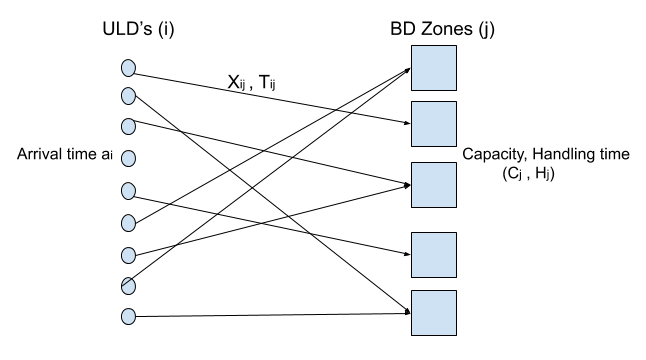
\includegraphics[width=12cm]{BDzone.png}\qquad

$\textcolor{black}{x_{ij}\in\{0,1\},\forall {i \in I, j \in J}}$ - denotes if ULD $i$ is
assigned to BD zone $j$ or not.


$\textcolor{black}{t_{j}}$ - Time taken to transport an ULD to BD
zone \textcolor{black}{$j$}

$\textcolor{black}{C_{j}}$ - Capacity of each BD Zone \textcolor{black}{$j$}

$\textcolor{black}{H_{j}}$ - Handling time of a ULD from in BD zone \textcolor{black}{$j$}

$\textcolor{black}{a_{i}+s_{i}+{\displaystyle \sum_{i,j\in E}x_{i,j}T_{j}}}$ - gives the
Arrival time of ULD \textcolor{black}{$i$} to its BD zone \textcolor{black}{$j$}

\pagebreak

\textbf{\underline{\large{Warehouse}}}:

\textbf {When the shipments are unpacked, they are sent to the storage warehouse (WH) which is fully automated and with the assumption, that there are never capacity issues in the storage WH. In a next step the shipments are built up again to ULDs depending on their connecting flight. A departing aircraft type has a link to a specific BU zone, so with the provided information which aircraft the shipment should go on, the BU zone is known.
}

$\newline$

$\textcolor{black}{T_{j}^{\prime}}$ - Time taken to transport shipment from BD zone \textcolor{black}{$j$} to Warehouse

$\textcolor{black}{W_{k}}$ - Time at which, all shipments for a new Flight k are requested

$\textcolor{black}{T_{k}^{\prime}}$ - Transport time from Warehouse to BU Zone for all shipments of Flight \textcolor{black}{$k$}

$\newline$

\textbf{\underline{\large{Build Up (BU) Zone}}}:

$\newline$

$\textcolor{black}{B_{k}}$ - Time taken to Build up ALL new ULDs for flight \textcolor{black}{$k$}

$\textcolor{black}{d_{k}}$ - Departure time of a flight \textcolor{black}{$k$} must be ready (given)

$\textcolor{black}{T_{k}}$ -Transport time from BU to Flight \textcolor{black}{$k$} (given)

$\textcolor{black}{p_{k}^{\prime}}$ - Default processing time of flight \textcolor{black}{$k$} (given)

$\textcolor{black}{p_{k}^{\prime\prime}}$ - Pre processing time of flight \textcolor{black}{$k$} (given)

$\textcolor{black}{W_{k}}$ + $\textcolor{black}{T_{k}}$ +${T_{k}^{\prime}}$+ $\textcolor{black}{B_{k}}$ + $\textcolor{black}{p_{k}^{\prime}}$ + $\textcolor{black}{p_{k}^{\prime\prime}}$ $\leq$ $\textcolor{black}{d_{k}}$ //Constraint respecting Flight time

$\newline$

\noindent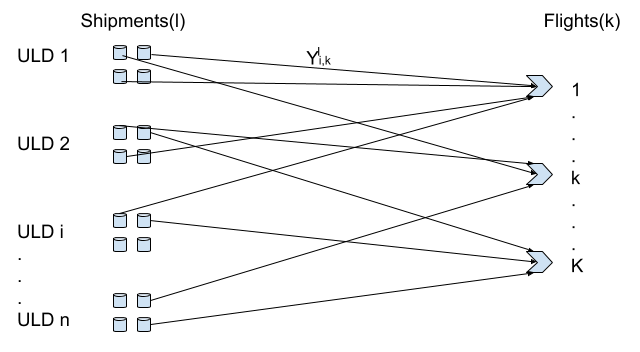
\includegraphics[width=12cm]{BUzone.png}\qquad

\pagebreak

Let $\textcolor{black}{Y_{i,k}^{l}}$ $\in\{0,1\}$ - depending on whether shipment l going to flight k is in ULD i or not.

$\textcolor{black}{w_{l}}$ - Weight of each shipment \textcolor{black}{$l$} (given)

$\textcolor{black}{Q_{k}}$ - Total weight of shipments going via flight \textcolor{black}{$k$} (summation of $\textcolor{black}{w_{l}}$)(given)

$\textcolor{black}{\displaystyle \sum_{i\in I} \sum_{l\in L}Y_{i,k}^{l}}$$\textcolor{black}{w_{l}}$ = $\textcolor{black}{Q_{k}}$ , $\forall{k}$ - Respecting assigned shipment weight to Flights \textcolor{black}{$k$}

$\textcolor{black}{\displaystyle \sum_{i\in I} \sum_{l\in L} \sum_{k\in K}Y_{i,k}^{l}}$ - N // Total no of shipments

All shipments of flight k, should reach be available before time $\textcolor{black}{W_{k}}$:

$\textcolor{black}{a_{i}+s_{i}+{\displaystyle \sum_{i,j\in E}x_{i,j}T_{j}}}+{T_{j}^{\prime}}+{H_{j}}$ $\leq$ ${W_{k}}$ + (1-${Y_{i,k}^{l}}$)M, $\forall{i,k,l}$ // Time constraint for every shipment.

\end{flushleft}

\end{document}
